
The symmetric group on four letters, $S_4$, contains the following permutations:

\begin{center}
\begin{tabular}{|c|c|}
\hline
permutations & type\\[4pt]
\hline
(12), (13), (14), (23), (24), (34) & 2-cycles \\[4pt]
(12)(34), (13)(24), (14)(23) & product of 2-cycles \\[4pt]
(123), (124), (132), (134), (142), (143), (234), (243) &  3-cycles \\[4pt]
(1234), (1243), (1324), (1342), (1423), (1432) & 4-cycles \\[4pt]
\hline
\end{tabular}
\end{center}

\begin{figure}[!ht]
\vspace{-9cm}
\hskip-1.5cm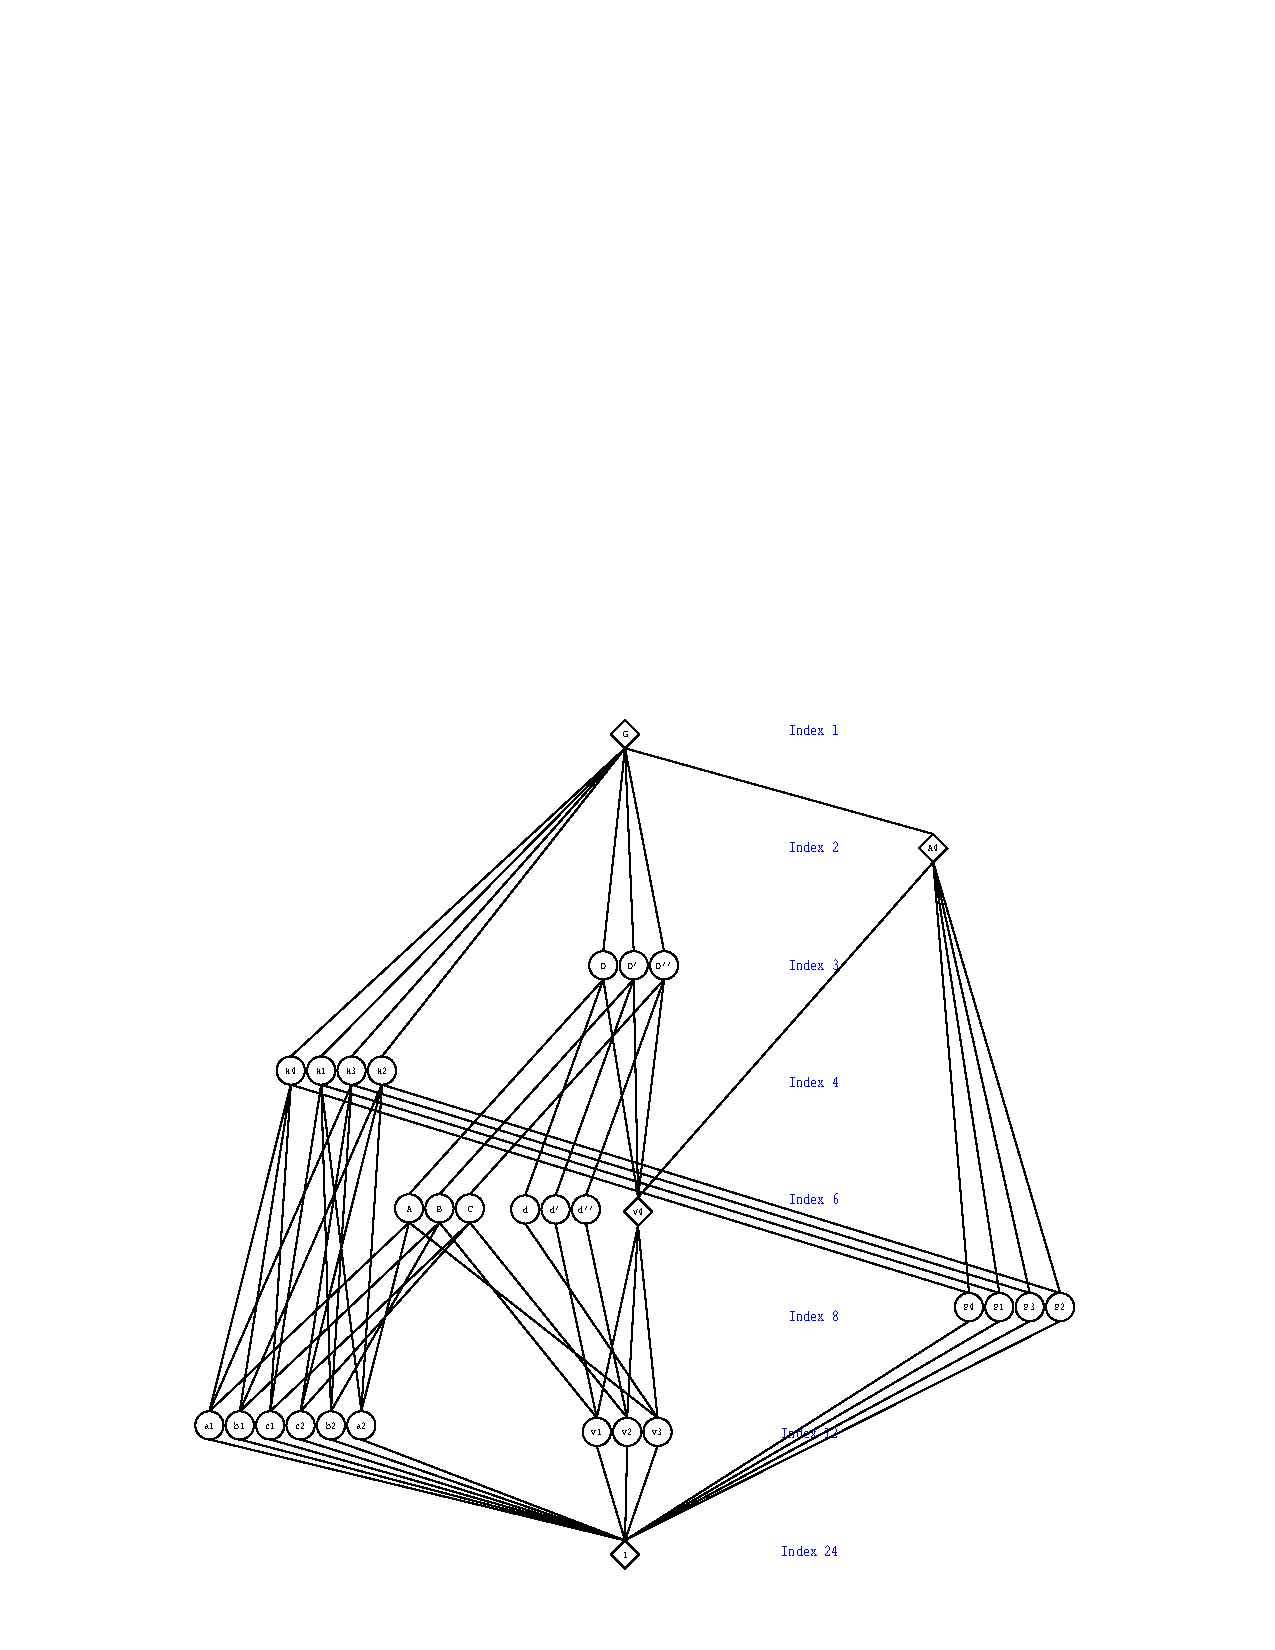
\includegraphics[height=20cm]{SubS4morelabels.pdf}%
\caption{Hasse diagram of $\Sub[S_4]$ drawn by the XGAP program.}
\label{fig:SubS4}
\end{figure}

~
\vfill

\newpage

{\footnotesize
    \begin{table}[h!]
      \centering
      \caption{There are 30 subgroups of $S_4$; all 
        except $(e)$ and $S_4$ are displayed here.}
      \begin{tabular}{|c|c|c|c|}
        \hline
        label & elements & order& isomorphic to\\
\hline
$A_4$ & $\{e, (12)(34), (13)(24), (14)(23),(123), (124), \ldots$& 12 & $A_4$\\[4pt]
      & $\ldots, (132), (134), (142), (143), (234), (243)\}$  & &\\[4pt]
\hline
$V_4$ & $\{e, (12)(34), (13)(24), (14)(23)\}$ & 4& $V_4$\\[4pt]
\hline
$v_1,\, v_2, \,v_3$ & $\{e, (12)(34)\},\; \{e, (13)(24)\}, \; \{e, (14)(23)\}$ & 2, 2, 2& $Z_2$\\[4pt]
\hline
$P_1$ & $\{e, (123), (132)\}$ & 3& $Z_3$\\[4pt]
\hline
$P_2$ & $\{e, (124), (142)\}$ & 3& $Z_3$\\[4pt]
\hline
$P_3$ & $\{e, (134), (143)\}$ & 3& $Z_3$\\[4pt]
\hline
$P_4$ & $\{e, (234), (243)\}$ & 3& $Z_3$\\[4pt]
\hline
$D$ & $\{e, (12),(12)(34), (13)(24), (14)(23), (34), (1324), (1423)\}$ & 8& $D_4$\\[4pt]
\hline
$d$ & $\{e, (12)(34), (1324), (1423)\}$ & 4& $Z_4$\\[4pt]
\hline
$D'$ & $\{e, (12)(34), (13), (13)(24), (14)(23), (24), (1234), (1432)\}$ & 8& $D_4$\\[4pt]
\hline
$d'$ & $\{e, (13)(24), (1234), (1432)\}$ & 4& $Z_4$\\[4pt]
\hline
$D''$ & $\{e, (12)(34), (13)(24), (14), (14)(23), (23), (1243), (1342)\}$ & 8& $D_4$\\[4pt]
\hline
$d''$ & $\{e, (14)(23), (1243), (1342)\}$ & 4& $Z_4$\\[4pt]
\hline
$H_1$ & $\{e, (12), (13), (23), (123), (132)\}$ & 6& $S_3$\\[4pt]
\hline
$H_2$ & $\{e, (12), (14), (24), (124), (142)\}$ & 6& $S_3$\\[4pt]
\hline
$H_3$ & $\{e, (13), (14), (34), (134), (143)\}$ & 6& $S_3$\\[4pt]
\hline
$H_4$ & $\{e, (23), (24), (34), (234), (243)\}$ & 6& $S_3$\\[4pt]
\hline
$A$ & $\{e, (12),(12)(34),(34) \}$ & 4& $V_4$\\[4pt]
\hline
$a_1,\, a_2$ & $\{e, (12)\}, \; \{e, (34) \}$ & 2, 2& $Z_2$\\[4pt]
\hline
$B$ & $\{e, (13), (13)(24),(24)\}$ & 4& $V_4$\\[4pt]
\hline
$b_1,\, b_2$ & $\{e, (13)\}, \; \{e, (24)\}$ & 2, 2& $Z_2$\\[4pt]
\hline
$C$ & $\{e, (14), (14)(23), (23)\}$ & 4& $V_4$\\[4pt]
\hline
$c_2, \, c_1$ & $\{e, (14)\}, \; \{e, (23)\}$ & 2, 2& $Z_2$\\[4pt]
\hline
      \end{tabular}
    \end{table}
}
